% ---------------------------------------------------------------------
%abstract template for the Junior Conference 2022
% ---------------------------------------------------------------------
\documentclass[12pt,a4paper]{article}


\usepackage[utf8]{inputenc}
\usepackage{amsmath}
\usepackage{amsfonts}
\usepackage{amssymb}
\usepackage[T1]{fontenc}
\usepackage[left=2cm,right=2cm,top=3cm,bottom=2cm]{geometry}
\usepackage[english, francais]{babel}
\usepackage{graphicx}
\usepackage{caption}
\captionsetup{font=small,skip=10pt}
\usepackage{fancyhdr} % Ajout du package fancyhdr
\pagestyle{fancy} % Utilisation du style de page fancy
\renewcommand{\LARGE}{\fontsize{20pt}{24pt}\selectfont}
\renewcommand{\large}{\fontsize{14pt}{16pt}\selectfont}
\usepackage{etoolbox}
\bibliographystyle{unsrt}
\patchcmd{\thebibliography}{\section*{\refname}}{\section*{\normalsize\refname}}{}{}


\setlength{\parindent}{2.5em}


% Redéfinition du style d'en-tête pour la première page
\fancypagestyle{firstpagestyle}{
    \fancyhf{} % Efface les en-têtes et pieds de page actuels
    \renewcommand{\headrulewidth}{0pt} % Supprime la ligne horizontale
    \fancyhead[L]{\vspace{-1.5cm}\begin{center}
\includegraphics[height=2.3cm]{entete.pdf}\end{center}}
}

\begin{document}

\thispagestyle{firstpagestyle} % Applique le style d'en-tête personnalisé à la première page

\begin{otherlanguage}{english}
% ---------------------------------------------------------------------
\vspace*{-0.8cm} 
\begin{center}
\textbf{\begin{LARGE}
Parametric Study of Acoustic Liners\\
\end{LARGE}
\bigskip
\vspace*{-0.1cm}
\begin{large}
\textit{\underline{LUCYSZYN Edward}$^1$, ALAMI Nabil$^1$ and PAIN DIT HERMIER Raphaël$^{1,2}$}
\end{large}}\\
\bigskip
$^1$ \textit{CentraleSupélec, second year of engineering curriculum}\\
%
$^2$ \textit{M1 Mathématiques fondamentales, Magistère d'Orsay}\\
%
\textit{Presenting author e-mail: edward.lucyszyn@student-cs.fr}
\end{center}
\medskip
% ---------------------------------------------------------------------

Nowadays, issues related to noise pollution are becoming increasingly prevalent, particularly due to the sound pollution generated by aircraft. To better understand this phenomenon, one can study sound absorption within an aircraft engine's reactor, equipped with sound-absorbing material known as acoustic liner, with the main objective to absorb more with less material. This study is based on various physical equations of fluid mechanics (Euler equation system), incorporating boundary conditions.
\vspace{-0.1cm}
\begin{center}
    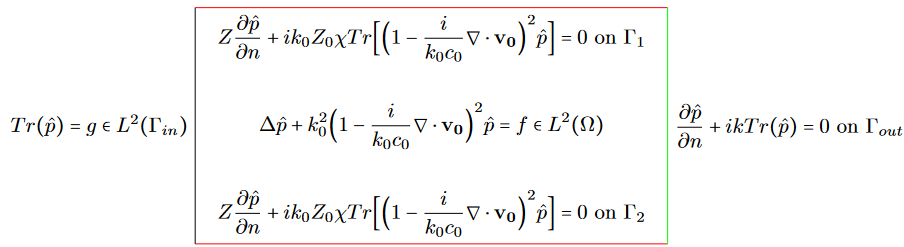
\includegraphics[width=17cm]{Resume_CONGRES_2024/GoodpictureEnglish.png}
\end{center}\par
\vspace{-0.1cm}
Several studies have addressed this type of problem using the Ingard-Myers condition [1], which allows for modeling sound absorption on the boundary where the liner is placed. However, several recent experiments have shown that this condition is not capable of precisely predicting the effect of an acoustic liner [2]. Nevertheless, there are several avenues to solve this problem. The study conducted by Y. Aurégan, R. Starobinski, and V. Pagneux in [3] leads to a modified Ingard-Myers condition involving a complex parameter $\beta_v$.\par
The study of the problem with this modified Ingard-Myers condition does not appear to have been widely explored in the scientific literature thus far. Therefore, we study the influence of $\beta_v$ on well-posedness of the problem and energy minimisation, supplemented by a numerical study of this parameter.


% ---------------------------------------------------------------------
%Keywords
\medskip
\noindent \textbf{Keywords: Acoustics, differential equations, Ingard-Myers conditions, acoustic liner, optimization.}\par
% -----------------------------------------------------------
%Supervisor
\medskip
\noindent \textbf{Supervisor:} Anna ROZANOVA-PIERRAT, MICS Laboratory, CentraleSupélec.\par
% ---------------------------------------------------------------------
% ---------------------------------------------------------------------
\vspace{-\baselineskip}
\begin{thebibliography}{1}
% ---------------------------------------------------------------------
\bibitem{1}
\label{1}
E. Luneville and J. -F. Mercier. {\em Mathematical modeling of time-harmonic aeroacoustics with a generalized impedance boundary condition}, 2012.

\bibitem{2}Ygaäl Renou, Yves Aurégana {\em Failure of the Ingard–Myers boundary condition for a lined duct: An experimental investigation}, 2011.

\bibitem{3}
Y. Aurégan, R. Starobinski,  V. Pagneux.
{\em Influence of grazing flow and dissipation effects on the acoustic boundary conditions at a lined wall}, 2011.

% ---------------------------------------------------------------------
\end{thebibliography}
% ---------------------------------------------------------------------
\end{otherlanguage}
% ---------------------------------------------------------------------
\newpage
\thispagestyle{firstpagestyle} % Applique le style d'en-tête personnalisé à la première page

\vspace*{-0.7cm} 
\begin{center}
\textbf{\begin{LARGE}
Étude Paramétrique d'un Liner Acoustique\\
\vspace*{-0.1cm}
\end{LARGE}
\bigskip
\begin{large}
\textit{\underline{LUCYSZYN Edward}$^1$, ALAMI Nabil$^1$ et PAIN DIT HERMIER Raphaël$^{1,2}$}
\end{large}}\\
\bigskip
$^1$ \textit{CentraleSupélec, deuxième année cursus ingénieur}\\
%
$^2$ \textit{M1 Mathématiques fondamentales, Magistère d'Orsay}\\
%
\textit{E-mail de l'auteur qui présente: edward.lucyszyn@student-cs.fr}
\end{center}
\medskip



% ---------------------------------------------------------------------

Les problèmes liés à la pollution acoustique se font de plus en plus nombreux de nos jours, notamment à cause de la pollution sonore générée par les avions. Pour mieux comprendre ce phénomène, il est possible d'étudier l'absorption sonore au sein d'un réacteur d'un avion, équipé sur les bords d'un matériau absorbant : le liner acoustique, avec comme objectif d'absorber plus avec moins de matériau. Cette étude se base sur diverses équations physiques de la mécanique des fluides (système d'équations d'Euler), dans lesquelles interviennent des conditions aux bords.\par
\vspace{-0.1cm}
\begin{center}
    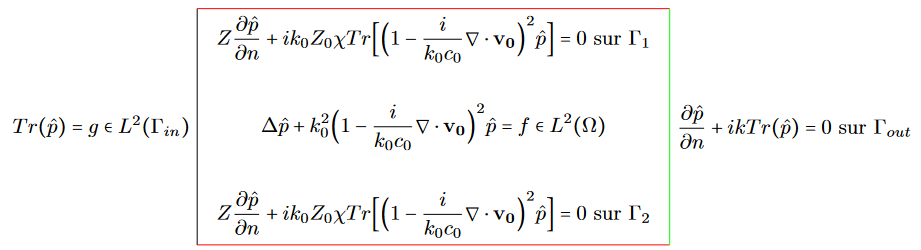
\includegraphics[width=17cm]{Resume_CONGRES_2024/Goodpicture.png}
\end{center}\par
\vspace{-0.1cm}
Plusieurs études ont traité ce type de problème avec la condition d'Ingard-Myers [1], qui permet de modéliser l'absorption sonore sur le bord où est posé le liner. Cependant, plusieurs expériences récentes montrent que cette condition n'est pas capable de prévoir précisément l'effet d'un liner acoustique [2]. Il y a cependant plusieurs voies pour résoudre ce problème. L'étude réalisée par Y. Aurégan, R. Starobinski, et V. Pagneux dans [3] permet d'aboutir à une condition d'Ingard-Myers modifiée faisant intervenir un paramètre $\beta_v$ complexe.\par
L'étude du problème avec cette condition d'Ingard-Myers modifiée semble ne pas avoir été largement explorée dans la littérature scientifique jusqu'à présent. Nous étudions alors l'influence de $\beta_v$ sur le caractère bien posé du problème et la minimisation d'énergie, complété par une étude numérique de ce paramètre.

% ---------------------------------------------------------------------
%Keywords
\medskip
\noindent \textbf{Mots-clés: Acoustique, équations différentielles, conditions d'Ingard-Myers, liner acoustique, optimisation.}\par

% ---------------------------------------------------------------------
%Encadrant
\medskip
\noindent \textbf{Encadrant:} ROZANOVA-PIERRAT Anna, Laboratoire MICS, CentraleSupélec. \par
% ---------------------------------------------------------------------
\vspace{-\baselineskip}
\begin{thebibliography}{1}
% ---------------------------------------------------------------------

% \bibitem{one}
% E. Redon, A.-S. Bonnet-Ben Dhia, J.-F. Mercier and S. Poernomo Sari {\em 
% Non-reflecting boundary conditions for acoustic propagation in ducts with acoustic treatment and mean flow}, 2011.

\bibitem{1}
E. Luneville and J. -F. Mercier. {\em Mathematical modeling of time-harmonic aeroacoustics with a generalized impedance boundary condition}, 2012.

\bibitem{2}Ygaäl Renou, Yves Aurégana {\em Failure of the Ingard–Myers boundary condition for a lined duct: An experimental investigation}, 2011.

\bibitem{3}
Y. Aurégan, R. Starobinski,  V. Pagneux.
{\em Influence of grazing flow and dissipation effects on the acoustic boundary conditions at a lined wall}, 2011.

% ---------------------------------------------------------------------
\end{thebibliography}
% ---------------------------------------------------------------------

% ---------------------------------------------------------------------

% ---------------------------------------------------------------------
\end{document}
% ---------------------------------------------------------------------
